\documentclass[12pt]{article}
\usepackage{setspace}
\setlength{\parindent}{4em}
\usepackage{fancyvrb}
\usepackage{graphicx}
\usepackage{geometry}
\renewcommand\thesection{\arabic{section}}
\renewcommand\thesubsection{\thesection.\arabic{subsection}}
\geometry{letterpaper, portrait, margin=1in}

%%%Title Page%%%
\title{\vspace{3cm}Lab 07\bigbreak Toy Processor with Memory on the Basys2 Board}
\author{
{\normalsize
\begin{tabular}{l r r}
 & \textbf{Ryan Cruz} & \textbf{Zachary Davis}\\
\textbf{Category} & ryan.cruz25@uga.edu & zachdav@uga.edu\\
\hline
Pre-lab 						  & 50 & 50\\
In-lab Module \& Testbench Design & 50 & 50\\
In-lab Testbench Sim. \& Analysis & 50 & 50\\
In-lab FPGA Synthesis \& Analysis & 50 & 50\\
Lab Report Writing 				  & 50 & 50\\
\end{tabular}
}}
%%%%%%%%%%%%%%%%%

\begin{document}
\maketitle
\newpage
\setstretch{2.5} % for custom spacing
\tableofcontents
\setstretch{1} % for custom spacing
\newpage

\section{Lab Purpose} \vspace{-.7cm} \line(1,0){470}
	\paragraph{}
		With the design of the toy processor complete, we can now implement it physically. With some tweaks to make it compatible, we can put it on the Basys2 board and load some simple programs onto it. 
		
\section{Implementation Details} \vspace{-.7cm} \line(1,0){470}
		
		
	\subsection{Part 1 - Clock and Bypass Circuits}

	\textbf{Clock}\\
	The clock for the processor, when implemented on the board, will be provided by the board. 
	This clock is too fast for human reading, so we will generate a push button clock and step through each operation.

		 \begin{figure}[h]
		 	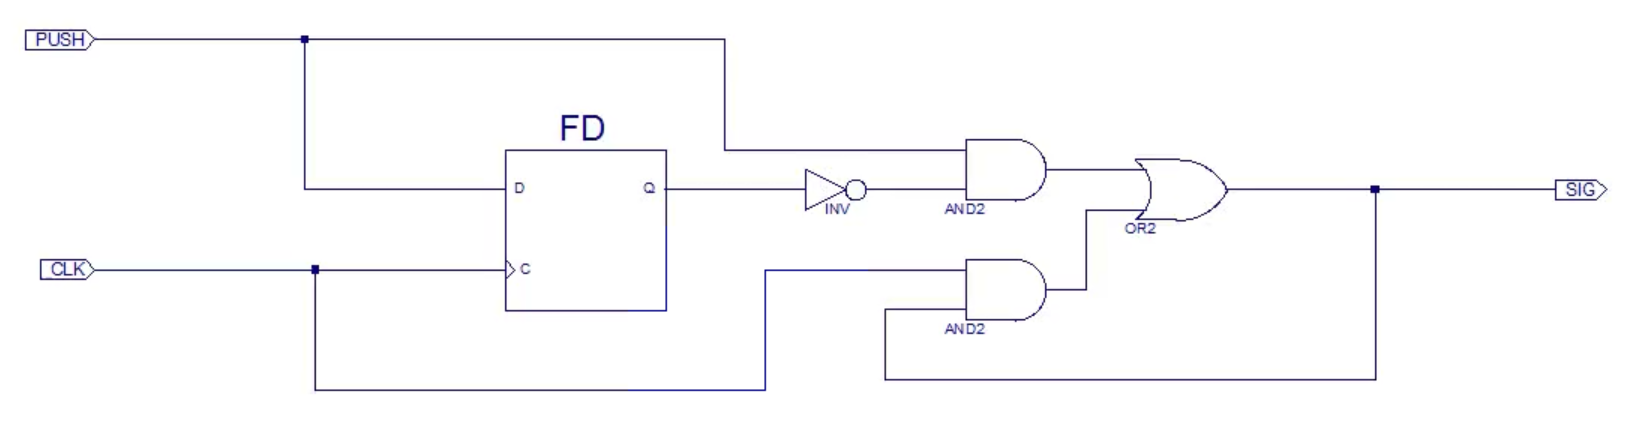
\includegraphics[scale=.55]{clk_signal_sch.PNG}
		 	\caption{Design of the clock signal created in Xilinx. (Designed on paper but just turned in a print out of this for prelab)}
		 \end{figure}

		
		\begin{Verbatim}[frame=single, fontsize= \small]
//Clock Testbench
`timescale 1ns/1ps

module clk_signal_tb;

	reg CLK = 1'b0;
	reg PUSH = 1'b0;

	wire SIG;

	initial // Clock process for CLK
		begin
			forever
			begin
				CLK = 1'b0;
				#100; 
				CLK = 1'b1;
				#100;
			end
		end
	
	clk_signal_sch UUT (
		.CLK(CLK),
		.PUSH(PUSH),
		.SIG(SIG));

	initial 
		begin

			#285;
			PUSH = 1'b1;
			#200;
			PUSH = 1'b0;
			#400;
			PUSH = 1'b1;
			#600;
			PUSH = 1'b0;

		end
endmodule

		\end{Verbatim}
		The test bench simply simulates button presses, and covers the test case of a holding the button as well. Results of the waveform are shown in the Expirimental Results section.\\\newline\textbf{Bypass}\\
		To avoid having to press the button 256 times to transition states, we designed a bypass so that the clock is automatic. 
		 \begin{figure}[h]
		 	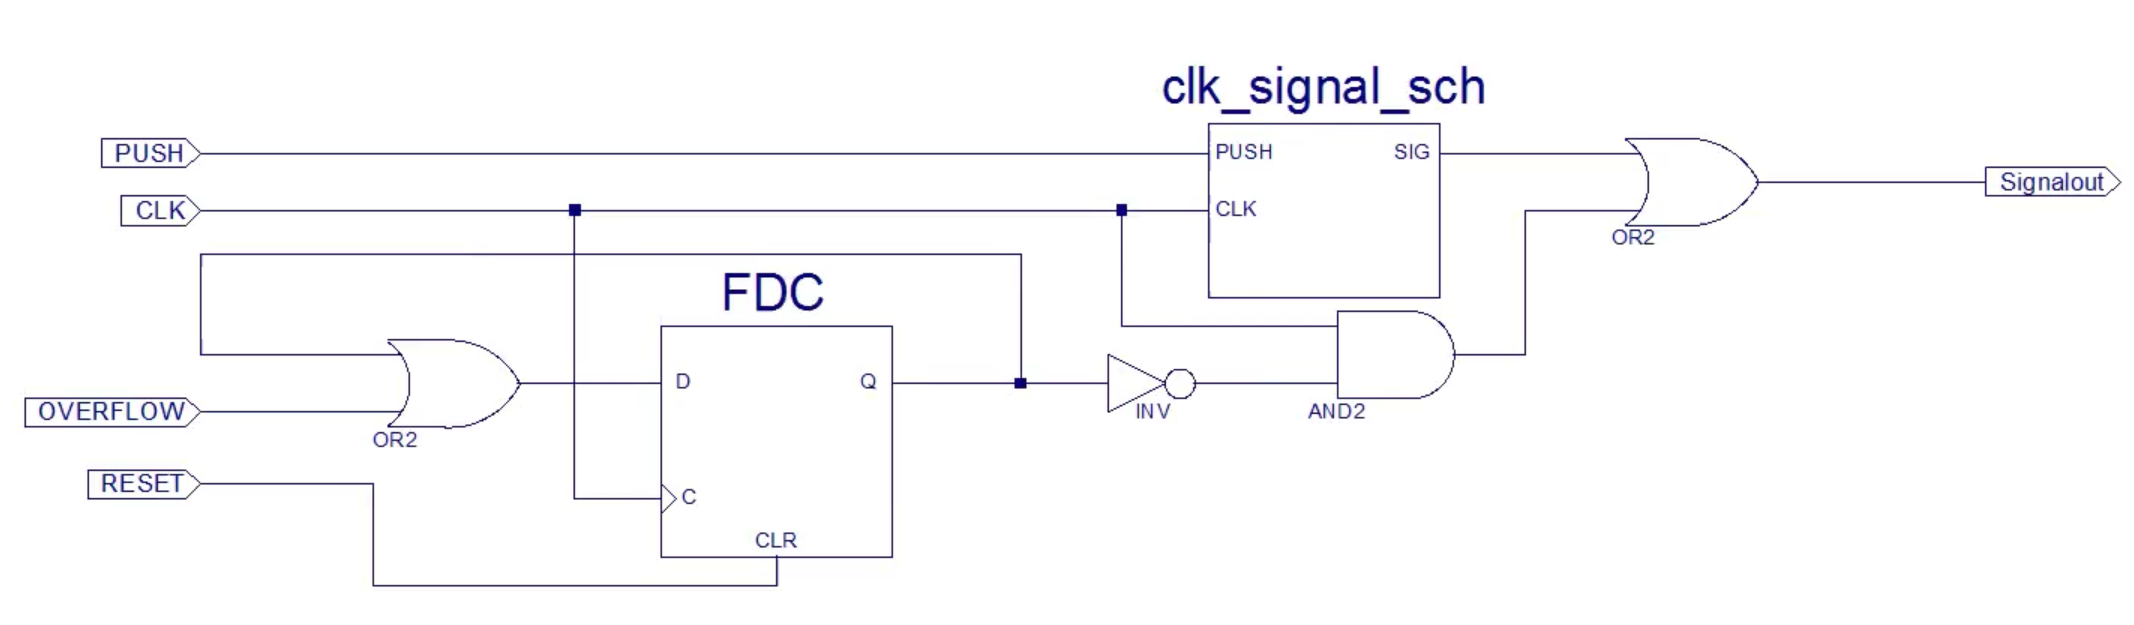
\includegraphics[scale=.45]{BypassClk.PNG}
		 	\caption{Design of the bypass clock signal created in Xilinx. (Designed on paper but just turned in a print out of this for prelab)}
		 \end{figure}
\begin{Verbatim}[frame=single, fontsize= \small]
`timescale 1ns/1ps

module BypassClk_tb;

	reg CLK = 1'b0;
	reg OVERFLOW = 1'b0;
	reg PUSH = 1'b0;
	reg RESET = 1'b0;
	
	wire Signalout;

	initial // Clock process for CLK
		begin
			forever
			begin
				CLK = 1'b0;
				#50; 
				CLK = 1'b1;
				#50;
			end
		end

	BypassClk UUT (
		.CLK(CLK),
		.OVERFLOW(OVERFLOW),
		.PUSH(PUSH),
		.RESET(RESET),
		.Signalout(Signalout));

	initial 
		begin
			// ------------- Current Time: 140ns
			#140;
			RESET = 1'b1;
			// -------------------------------------

			// ------------- Current Time: 340ns
			#200;
			RESET = 1'b0;
			// -------------------------------------
			
			// ------------- Current Time: 440ns
			#100;
			PUSH = 1'b1;
			// -------------------------------------

			// ------------- Current Time: 640ns
			#200;
			PUSH = 1'b0;
			// -------------------------------------

			// ------------- Current Time: 740ns
			#100;
			PUSH = 1'b1;
			// -------------------------------------

			// ------------- Current Time: 840ns
			#100;
			PUSH = 1'b0;
			// -------------------------------------

			// ------------- Current Time: 940ns
			#100;
			OVERFLOW = 1'b1;
			// -------------------------------------

			// ------------- Current Time: 1040ns
			#100;
			OVERFLOW = 1'b0;
			// -------------------------------------

			// ------------- Current Time: 2140ns
			#200;
			PUSH = 1'b1;
			// -------------------------------------

			// ------------- Current Time: 2340ns
			#200;
			PUSH = 1'b0;
			#100;
			PUSH = 1'b1;
			#100;
			PUSH = 1'b0;
			// -------------------------------------
		end
endmodule
\end{Verbatim}


		\newpage
		\subsection{Part 2 - Programming the Basys2 Board}
		To make the processor compatible with the board and for it to be testable, we must program the seven segment display, similar to how we have done in previous labs. It will display the instructions, as well as the accumulator.

		 \begin{figure}[h]
		 	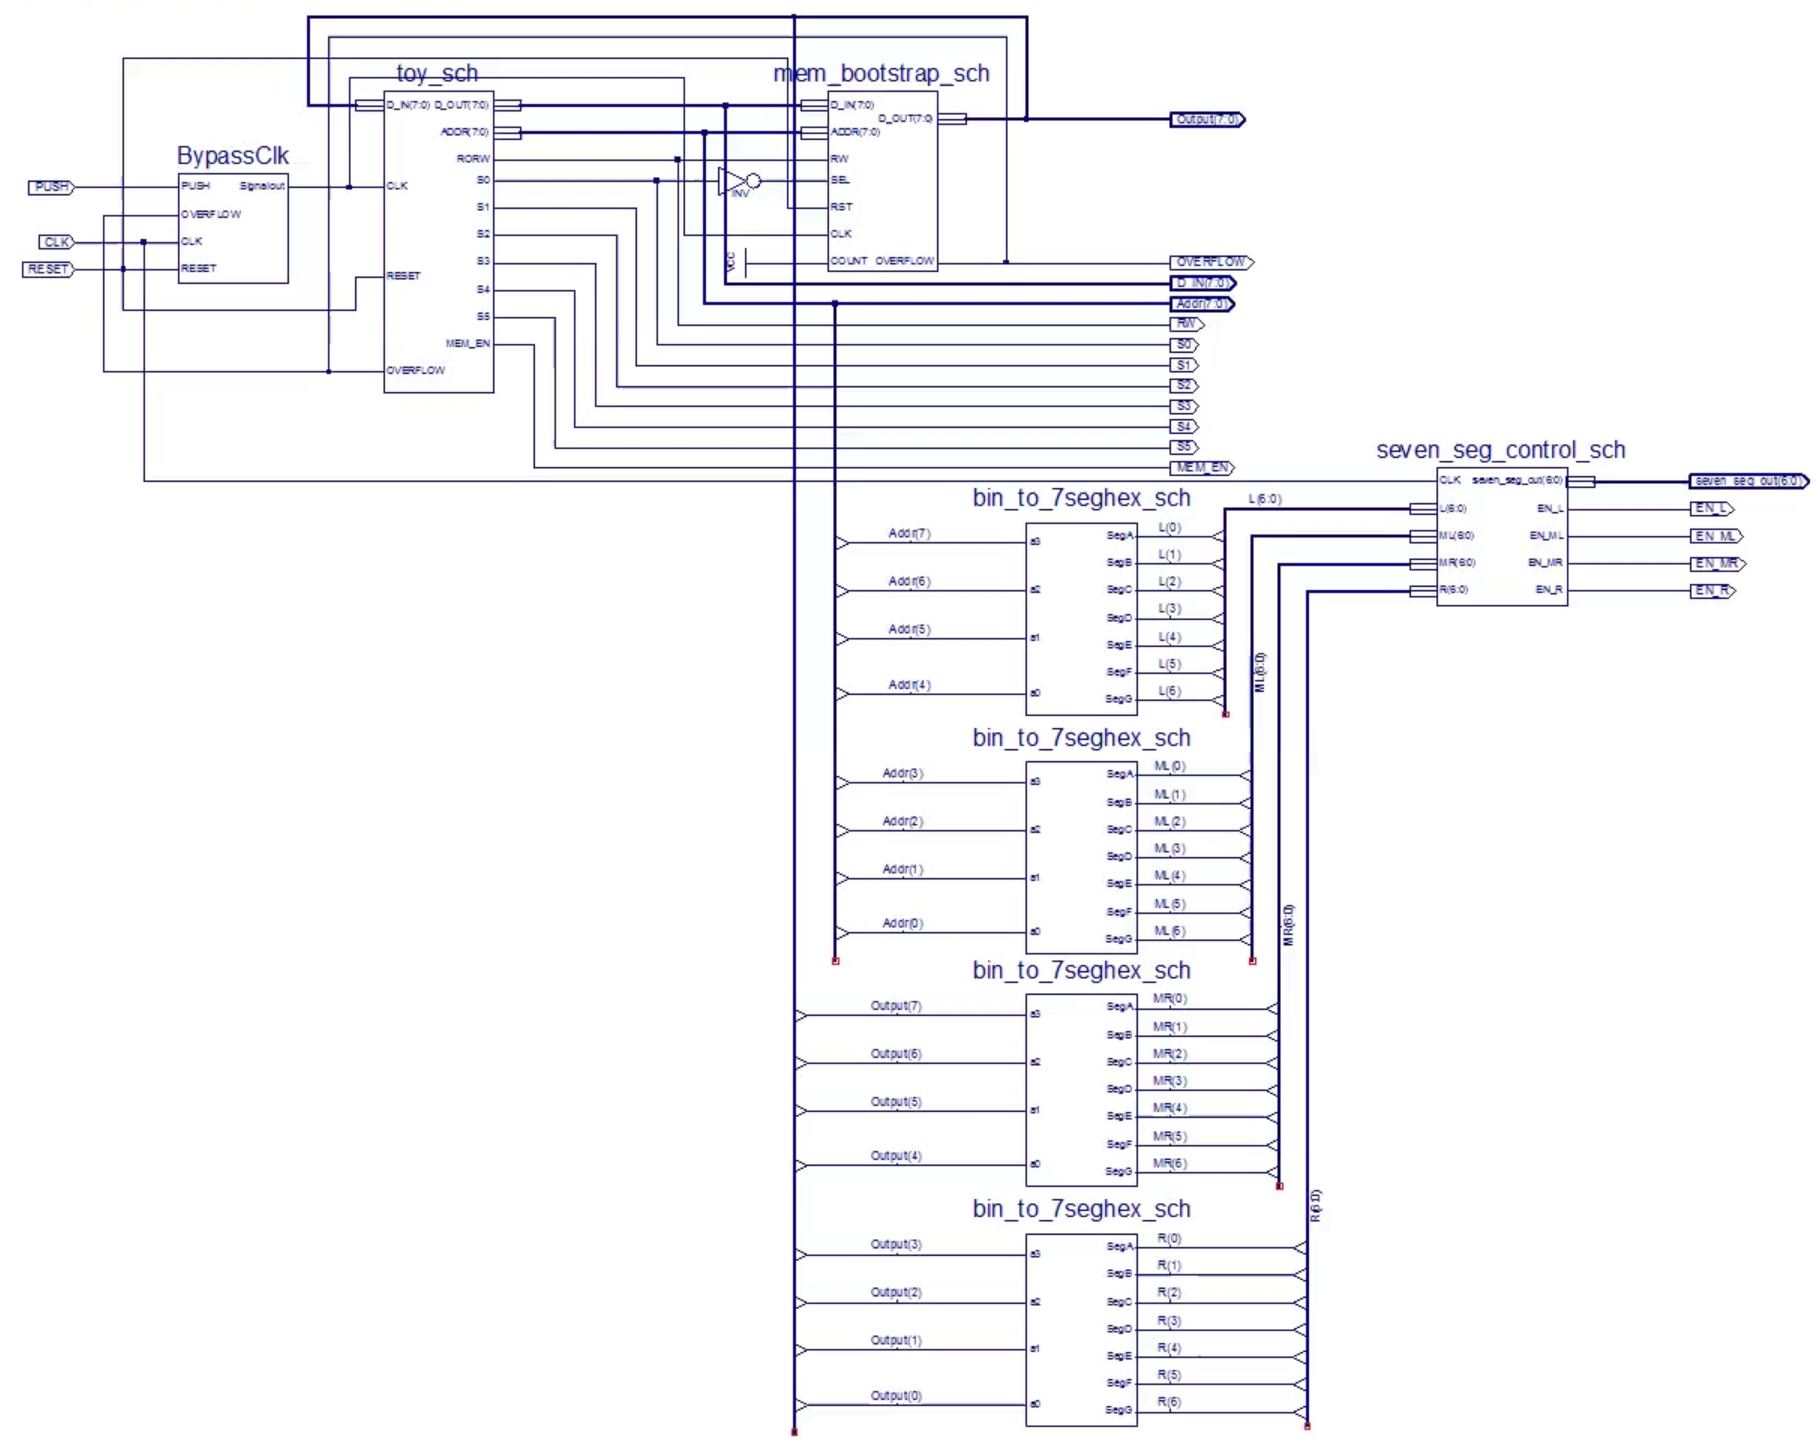
\includegraphics[scale=.5]{toyProcessor_Overall.PNG}
		 	\caption{Modifications to the ToyProcessorOverall schematic to add the seven segment displays.}
		 \end{figure}
\newpage

With the board ready for programs, we can now enter machinecode into ROM and actually see its output on the seven segment display. We will design two programs, with the 2nd testing all of the capabilities of our ToyProcessor.\\

The first program that we will load onto the board simply sums the numbers from 1-9 using the ADD instruction and then stores that sum. This program is not self-modifying, does not loop, and is linear -- it ends after the first run.
\begin{center}
\textbf{First Serial Addition Program}\\
\begin{tabular}{|l|l|l|}
\hline
Address & Instruction & Description\\
\hline
0       & 100	&CLR    \\
1       & 1		&ADD    \\
2       & 1		&1      \\
3       & 1		&ADD    \\
4       & 10	&2      \\
5       & 1		&ADD    \\
6       & 11	&3      \\
7       & 1		&ADD    \\
8       & 100	&4      \\
9       & 1		&ADD    \\
10      & 101	&5      \\
11      & 1		&ADD    \\
12      & 110	&6      \\
13      & 1		&ADD    \\
14      & 111	&7      \\
15      & 1		&ADD    \\
16      & 1000	&8      \\
17      & 1		&ADD    \\
18      & 1001	&9      \\
19      & 10000	&STORE 	\\
20      & 45	&45		\\
\hline
\end{tabular}
\end{center}

\begin{center}
\newpage
\textbf{Second Serial Addition Program}\\

\begin{tabular}{|l|l|l|}
\hline
Address & Instruction & Description \\
\hline
0       & 100	&CLR       \\
1       & 1		&ADD           \\
2       & 1010	&10        \\
3       & 10	&SUB         \\
4       & 1		&1          \\
5       & 10000	&STORE       \\
6       & 10	&2          \\
7       & 1000	&BNZ        \\
8       & 10010	&18       \\
9       & 1 	&ADD          \\
10      & 0		&0           \\
11      & 10000	&STORE       \\
12      & 1010	&10        \\
13      & 10000	&STORE       \\
14      & 1100100	&100     \\
15      & 100	&CLR         \\
16      & 1000	&BNZ        \\
17      & 1   	&1        \\
\hline
\end{tabular}
\end{center}


\newpage			
\section{Experimental Results}\vspace{-.7cm} \line(1,0){470}

\begin{center}
	% 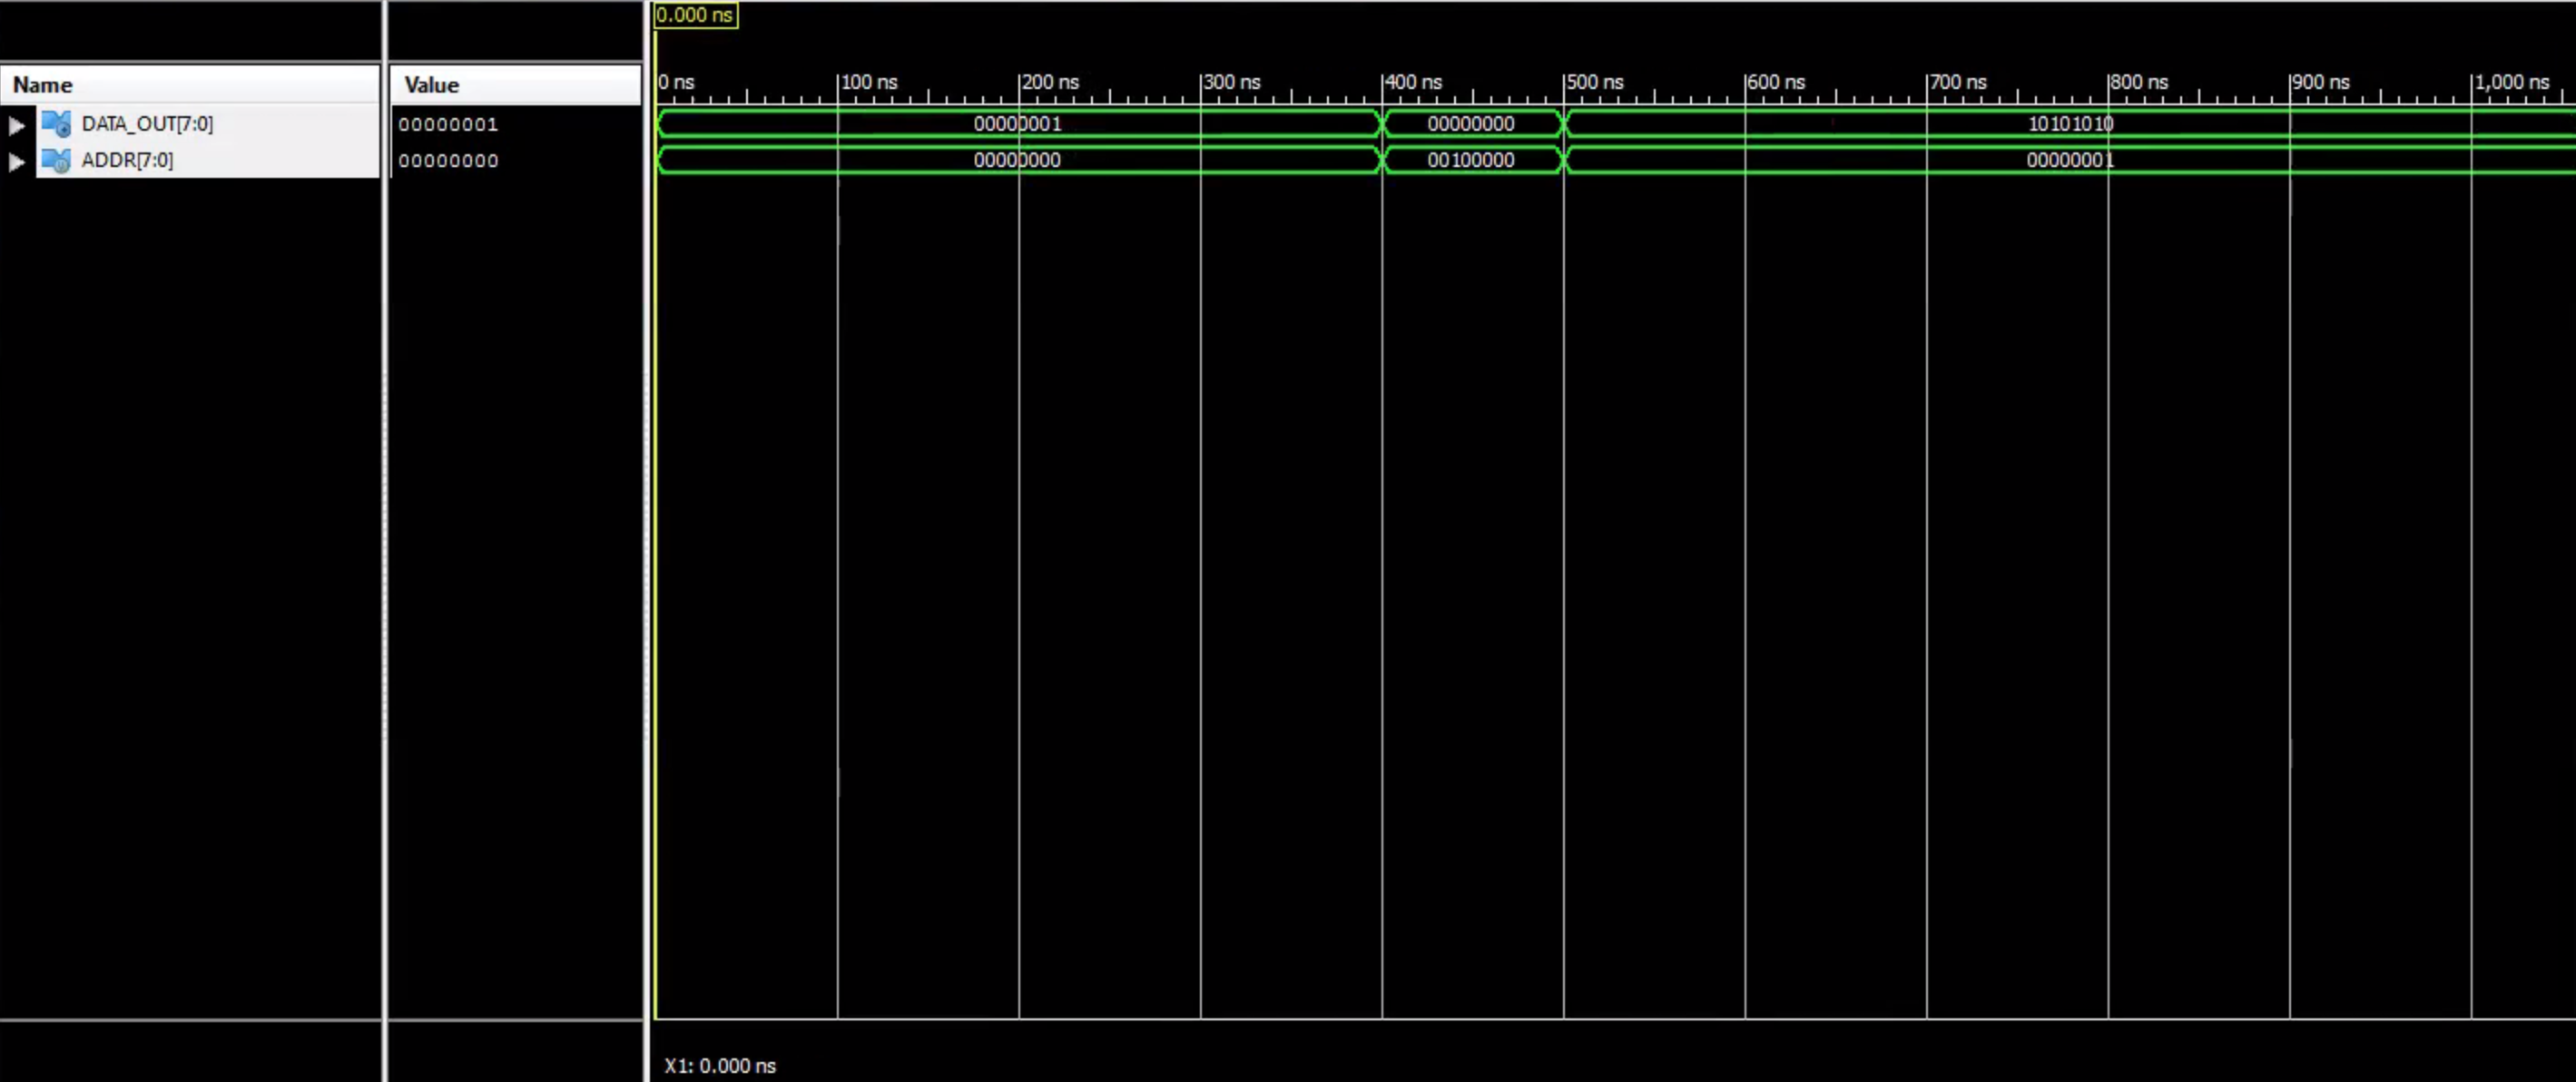
\includegraphics[scale=.3]{ROM_tb.png}\\
	% This is our ROM testbench and using the chart above in the ROM section you can match the addresses with the output given.\\
	% 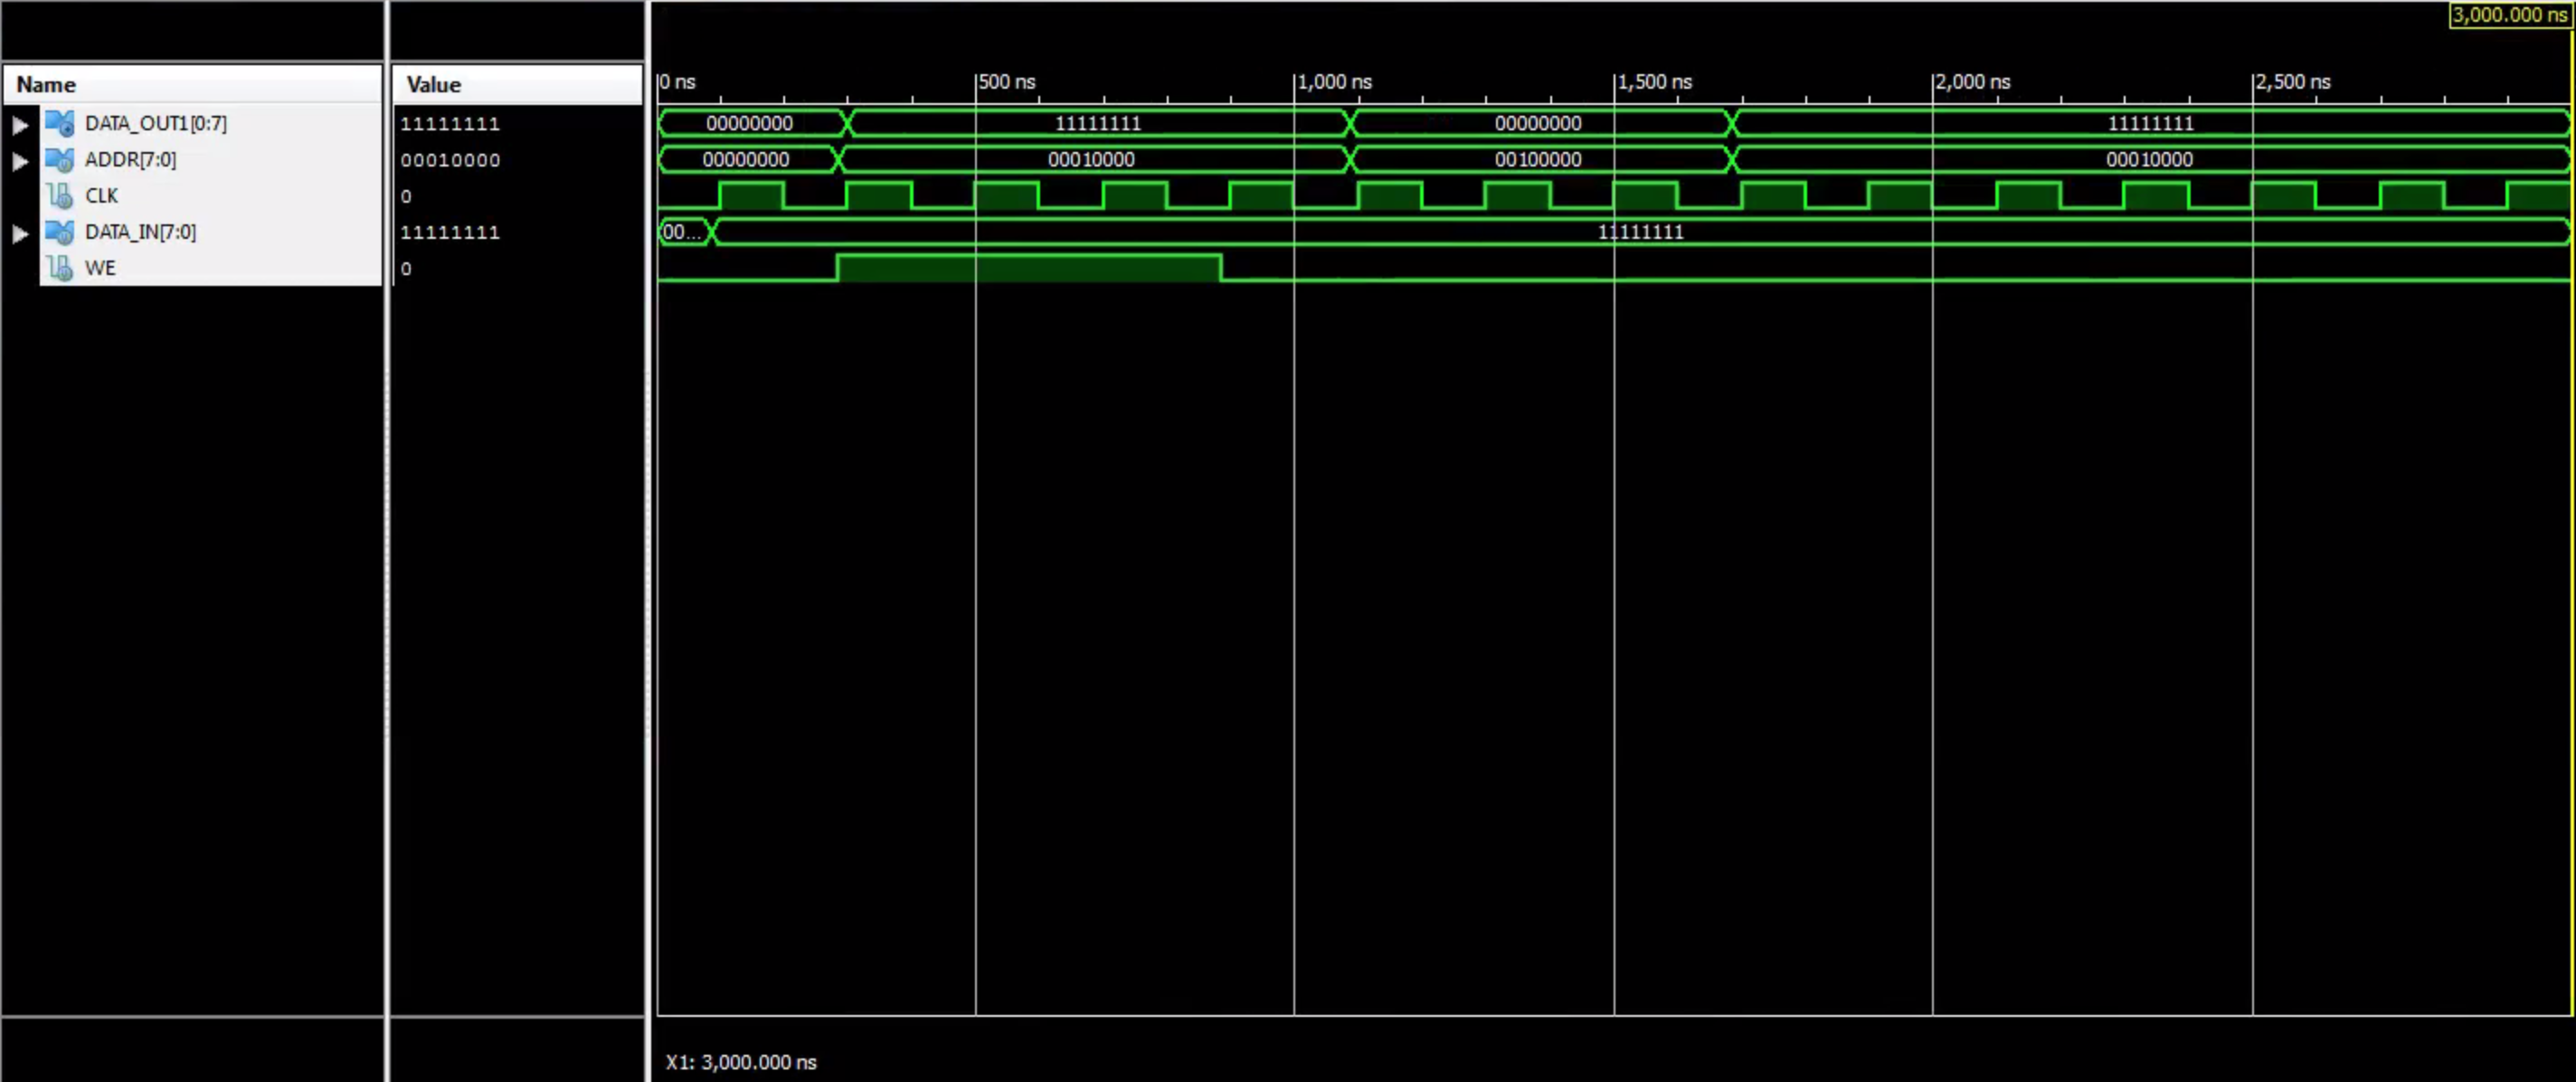
\includegraphics[scale=.3]{RAM_tb.png}\\
	% This is out RAM testbench and you can again see and verify what is stored in the tested address as well as se us write something to RAM. It is worth noting that nothing is actually written until WE goes high.\\
	% \newpage
	% 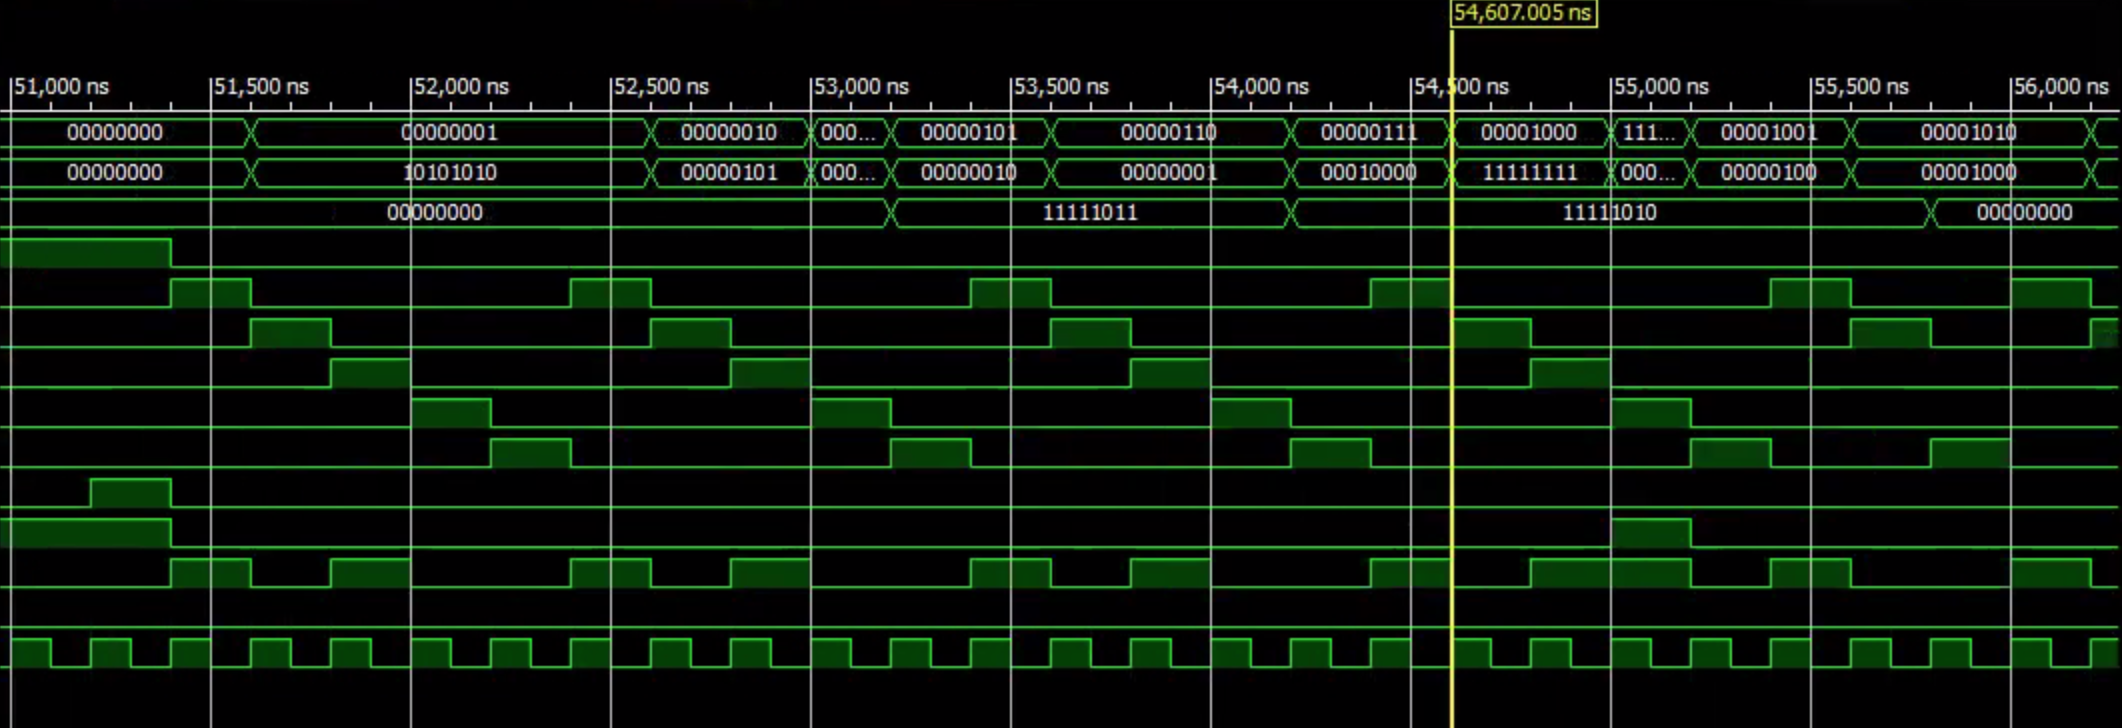
\includegraphics[scale=.4]{tb1.png}
	% 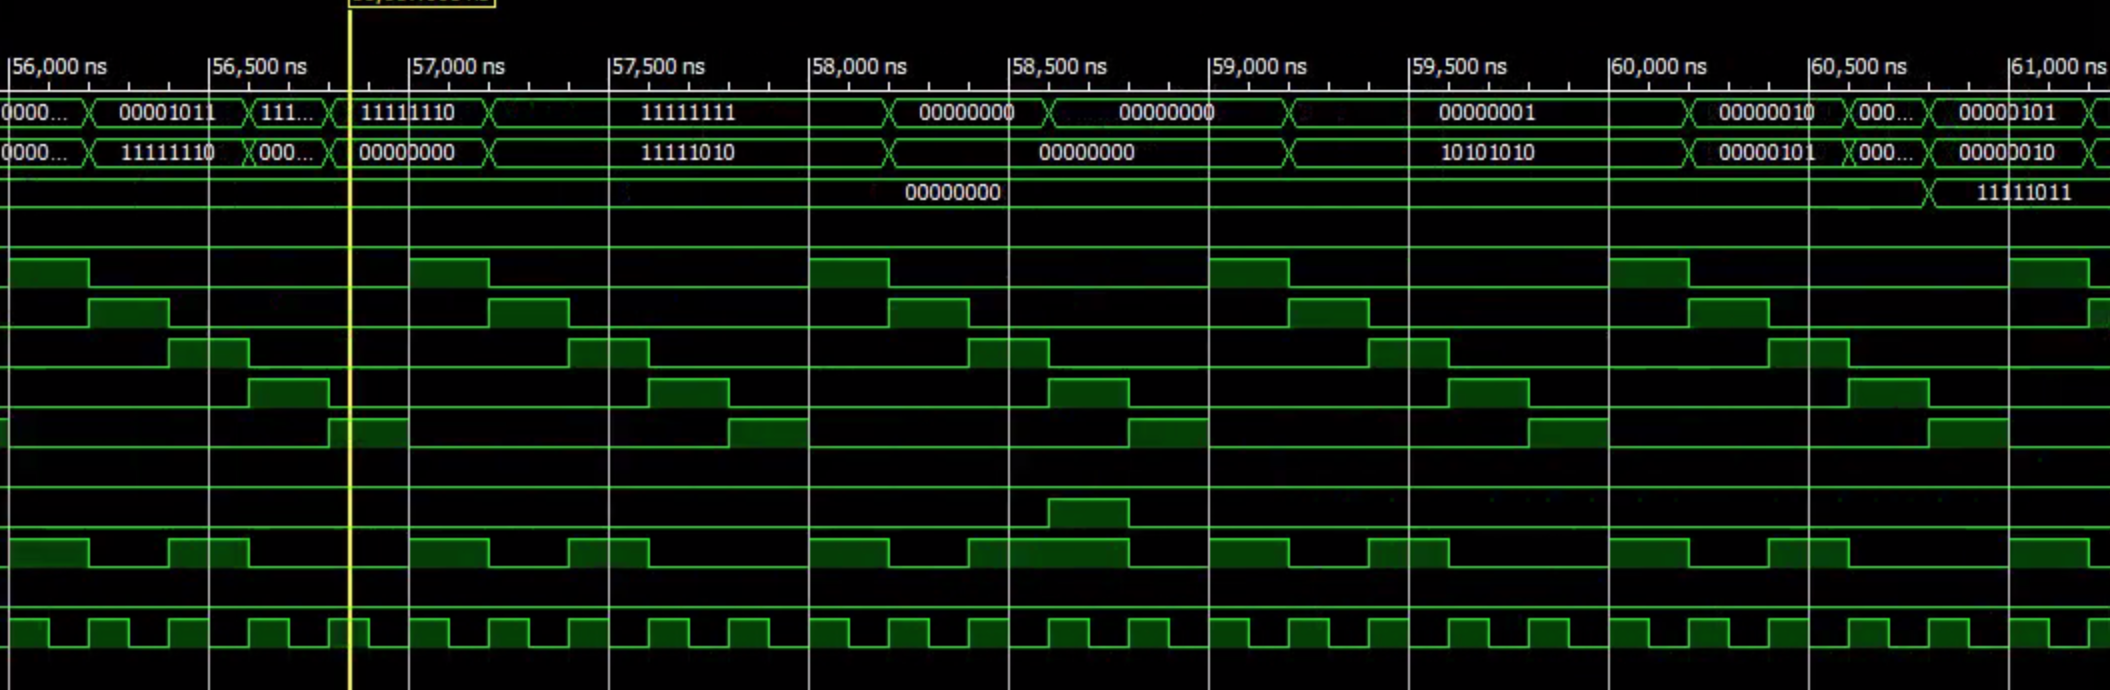
\includegraphics[scale=.4]{tb2.png}
	% 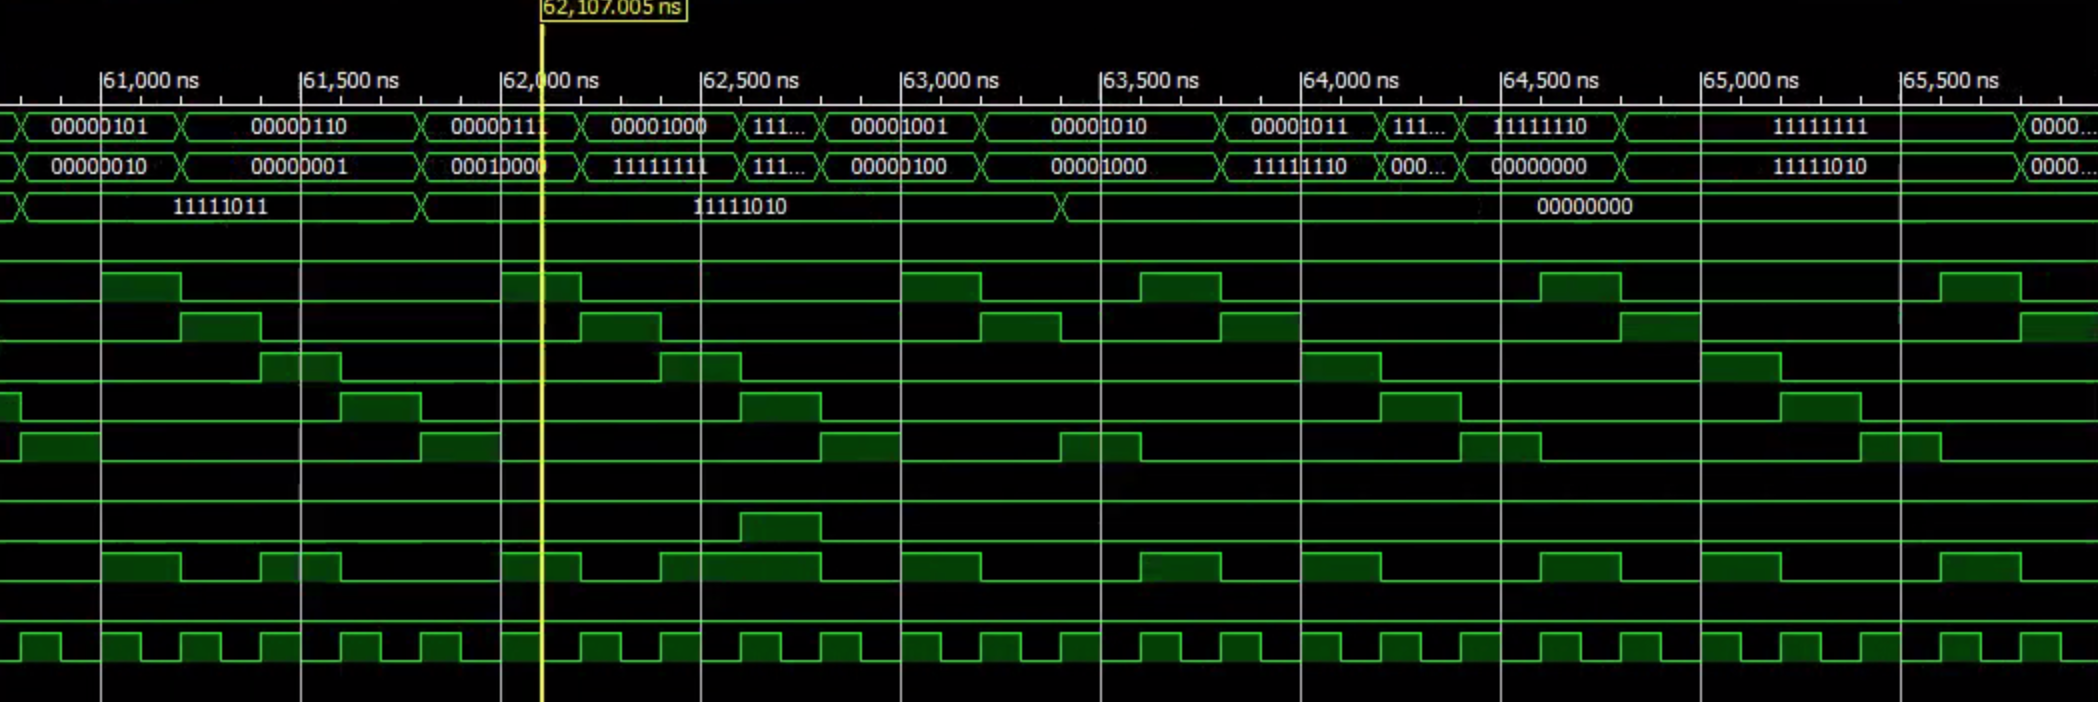
\includegraphics[scale=.4]{tb3.png}
	% 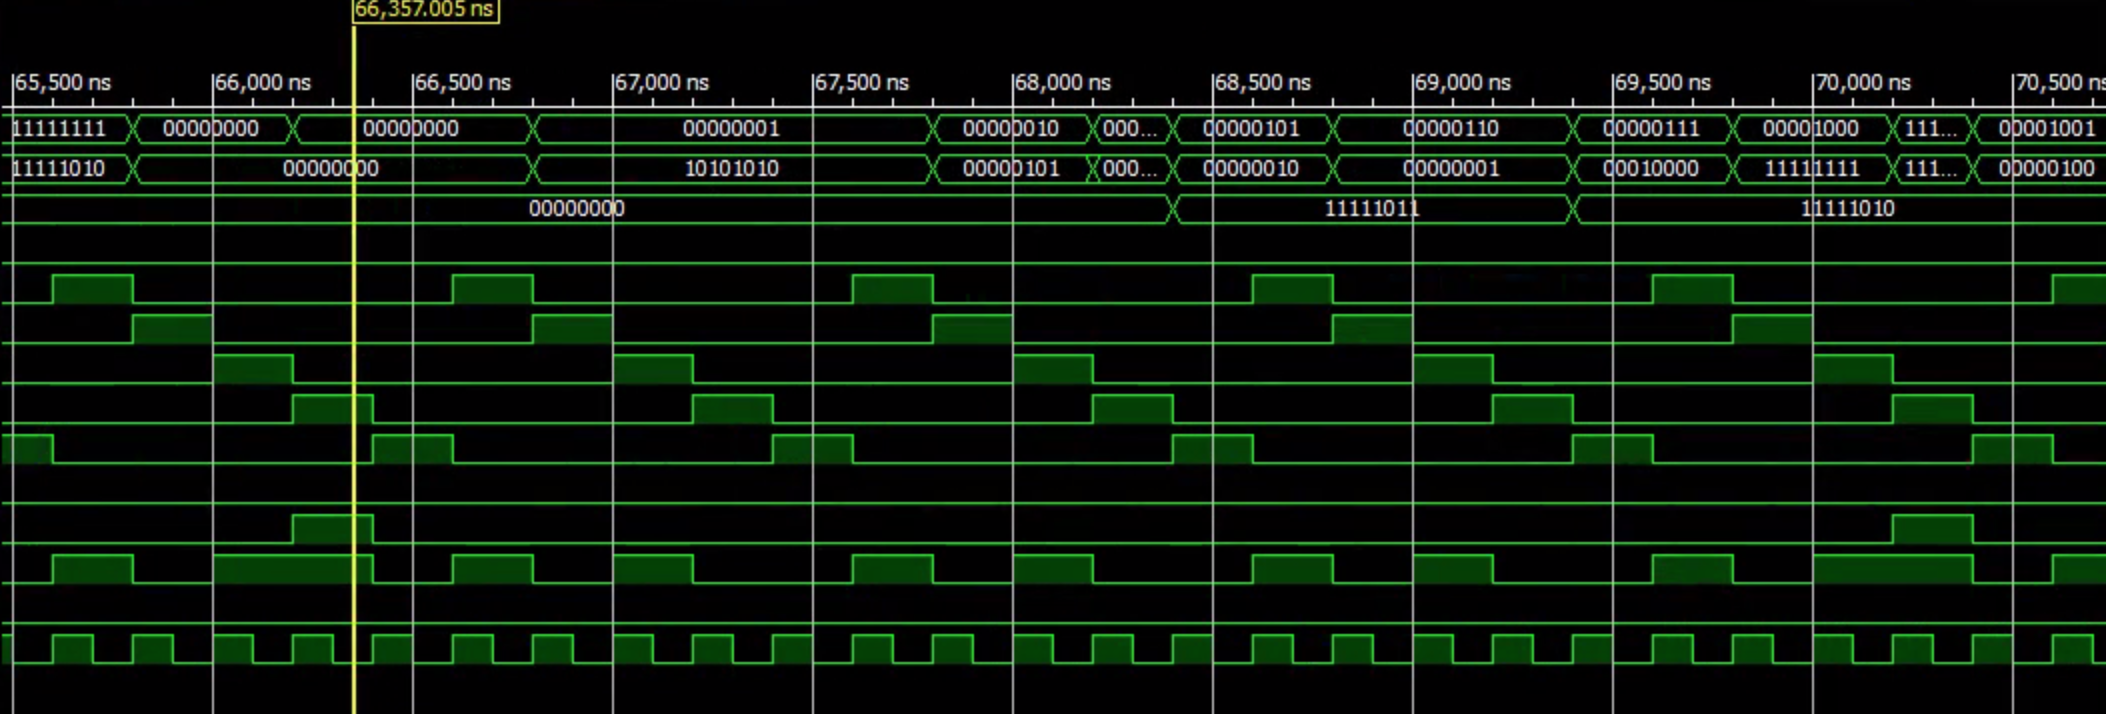
\includegraphics[scale=.4]{tb4.png}\\
	
\end{center}

	\newpage
\section{Significance} \vspace{-.7cm} \line(1,0){470}
	\paragraph{} 
		With memory added, we have much more flexibility with what we can input to the Toy Processor. Also, it is 

 \section{Comments/Suggestions}\vspace{-.7cm} \line(1,0){470}
 	\paragraph{} 
 		N.A.
		
\end{document}


